%!TEX root = ../../../../thesis.tex
\section{\textit{Physarum Polycephalum}}

	\Pp is an acellular slime mold and belongs to myxomycetes. It is native to the forests of France, Italy, Spain, Romania, North-, Middle- and South America as well as China, Nepal, Southeast Asia and Japan, see \Fref{fig:exploration:forest}. In the recent past \P has become increasingly at home in laboratories and schools across the globe where its extraordinary properties fascinate scientists and students alike, see \Fref{fig:exploration:lab}.

	\begin{figure}
		\centering
		\subfloat[\P exploring the forest][]{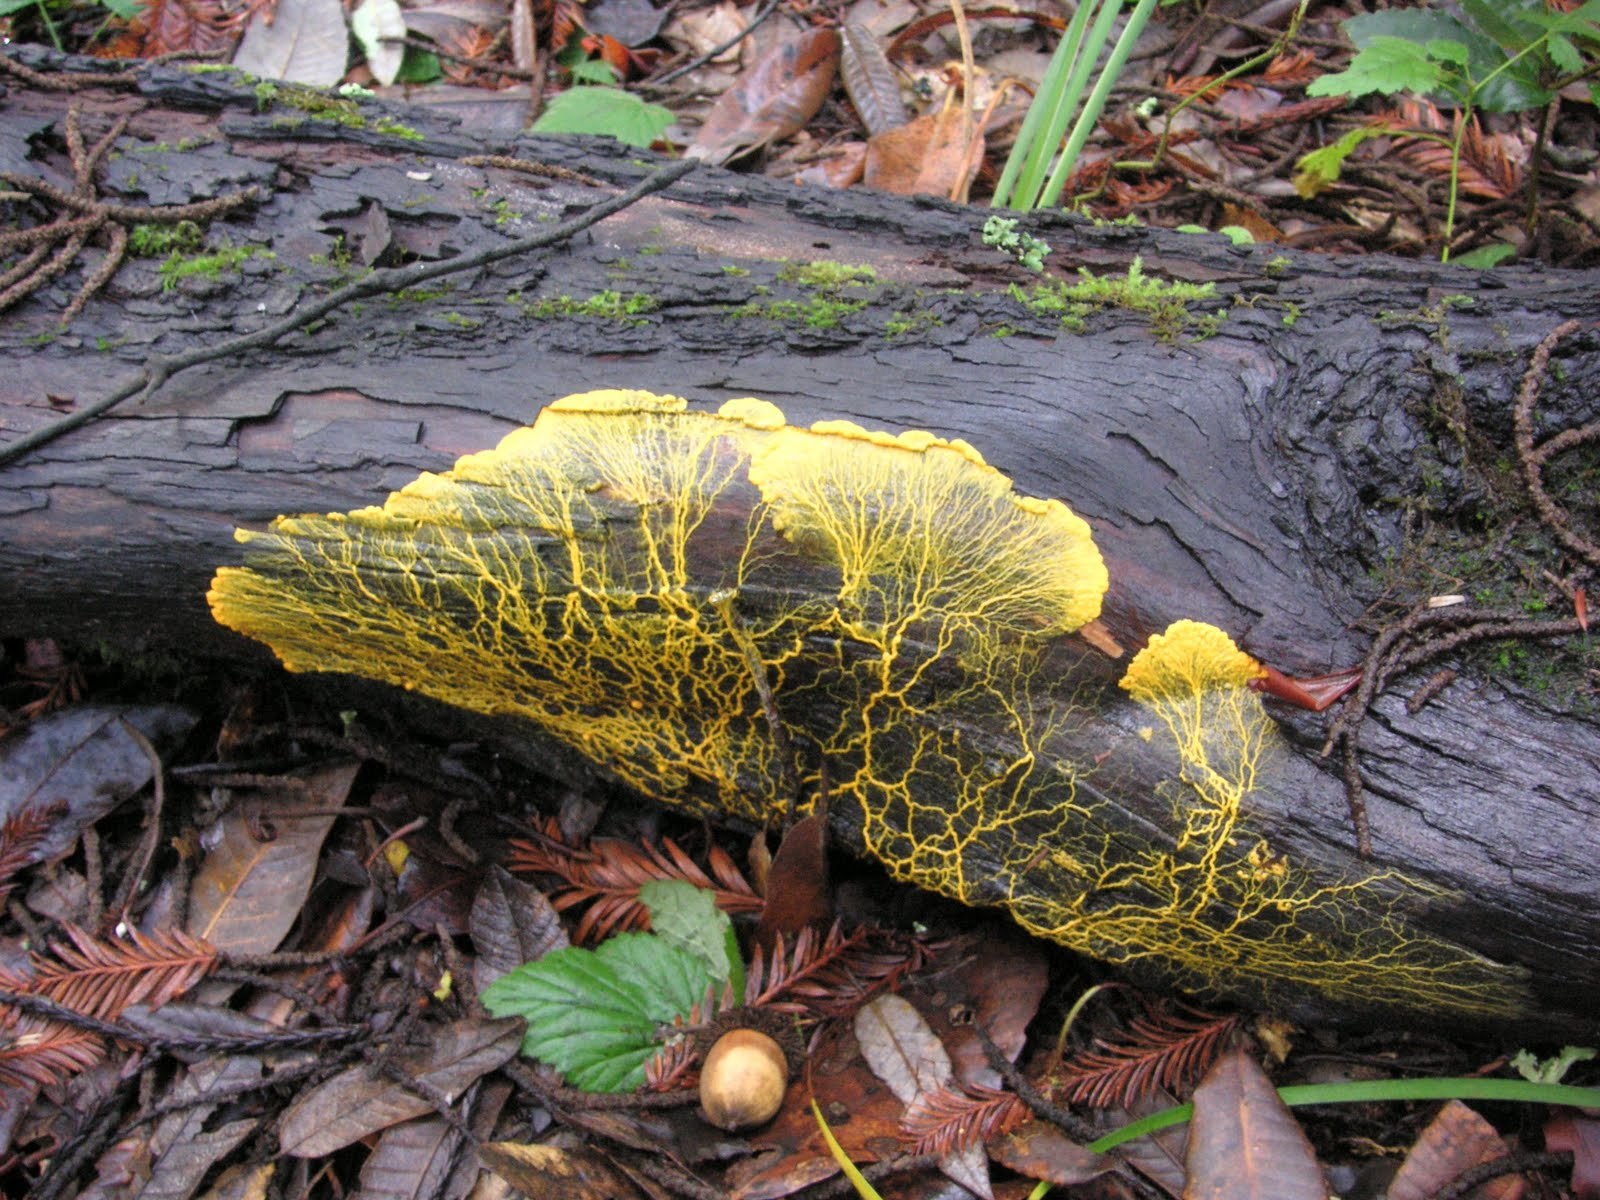
\includegraphics[width=0.5\linewidth,keepaspectratio]{physarum_exploring_forest.jpg}\label{fig:exploration:forest}}
		\subfloat[\P exploring the lab][]{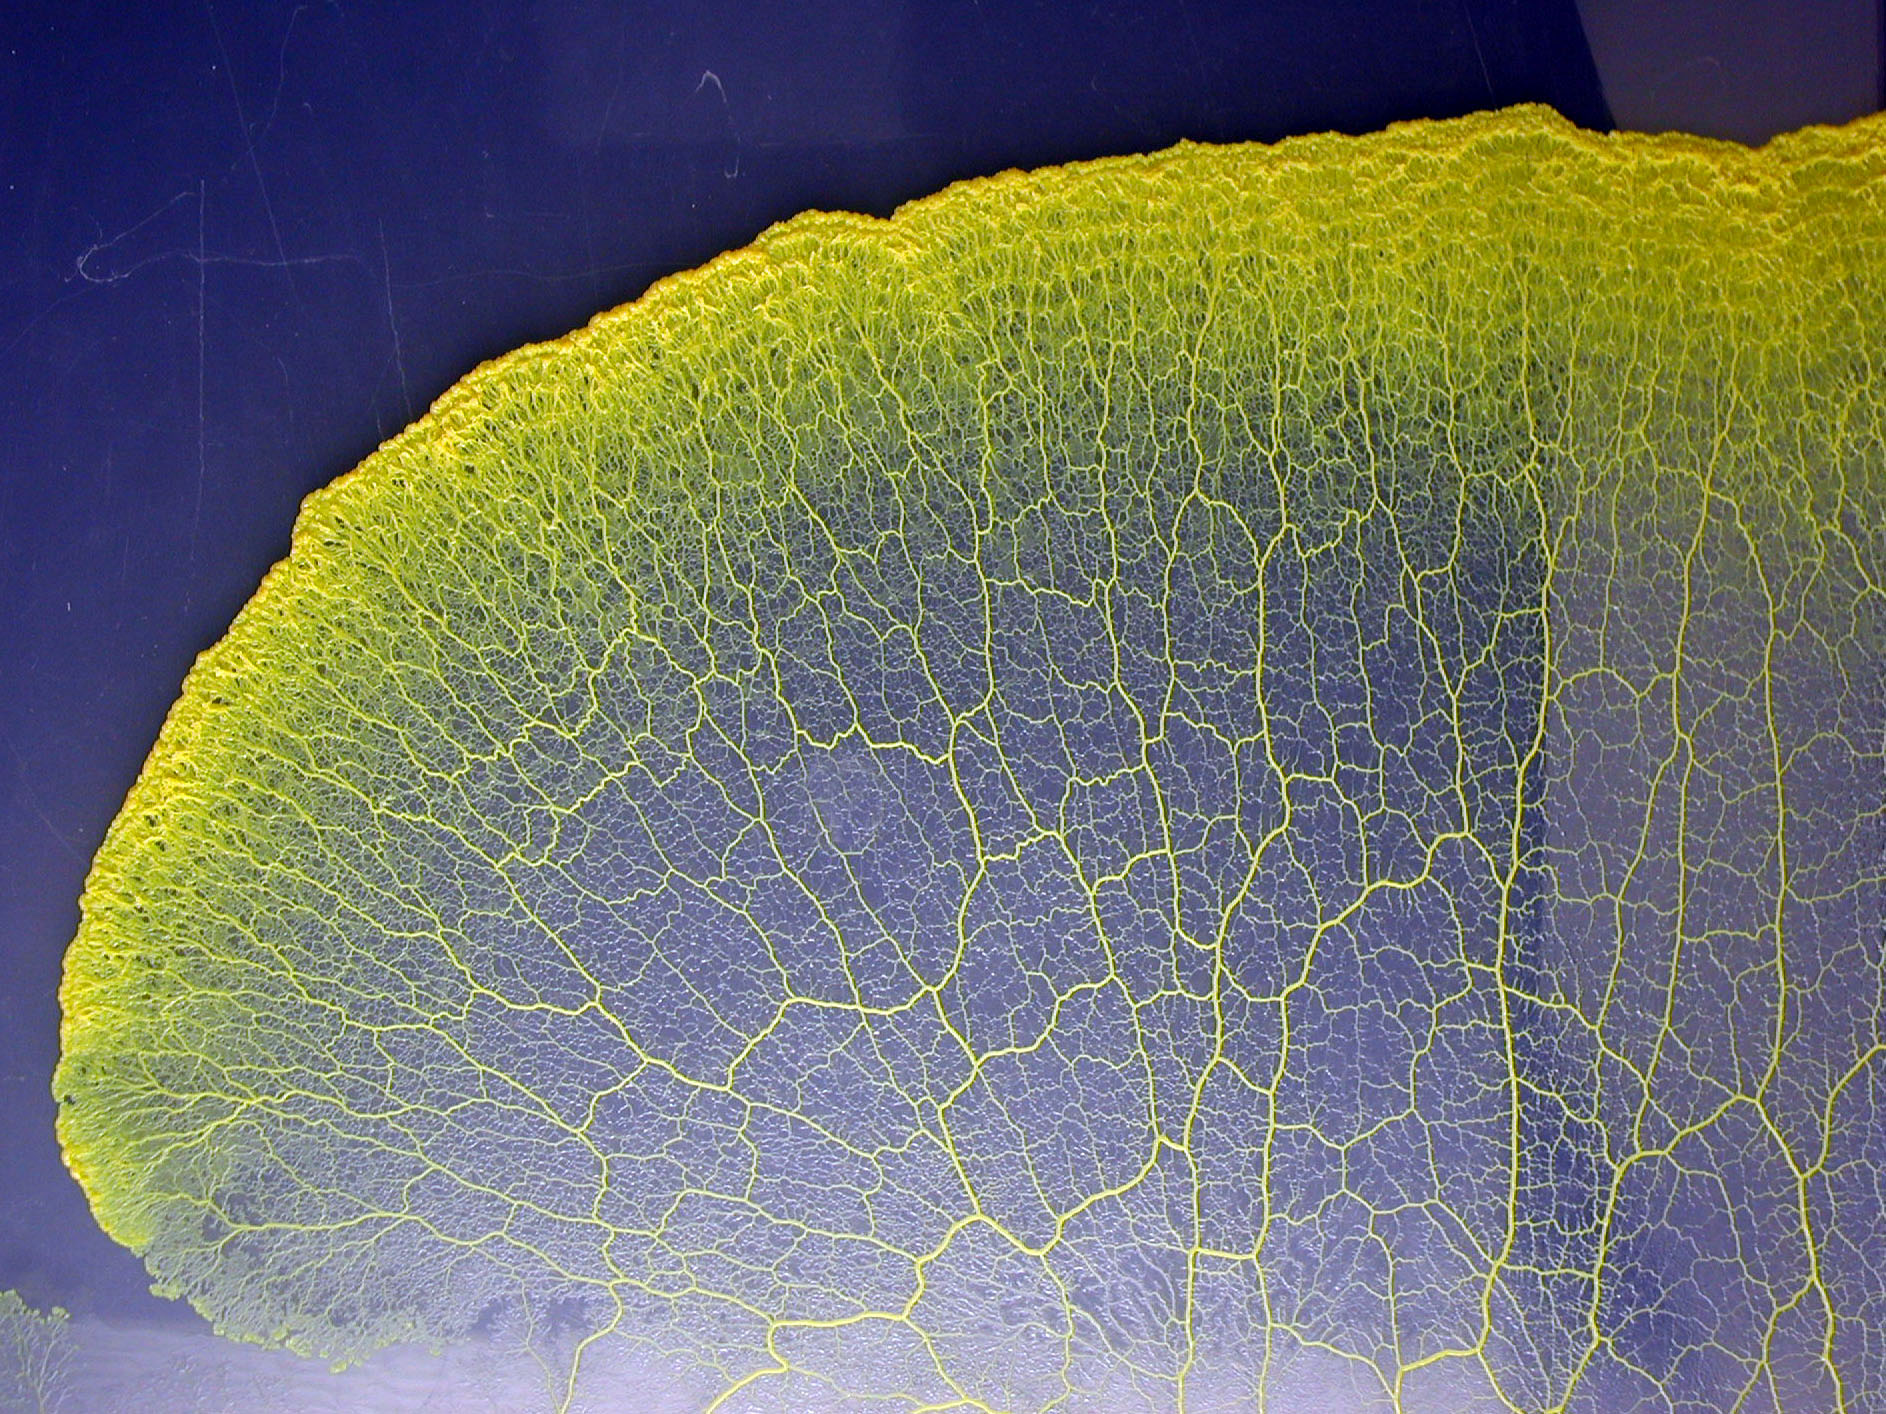
\includegraphics[width=0.5\linewidth,keepaspectratio]{physarum_exploring_petri_dish.jpg}\label{fig:exploration:lab}}
		\caption[\P exploring various environments]{\P is equally at home in the forest and the in the laboratory. Figures courtesy of Prof.~T.~Ueda, Hokkaido University.}
		\label{fig:exploration}
	\end{figure}

	In the following sections we give a basic introduction to \P and discuss its scientific importance. We summarize selected material form several sources that provide more detailed surveys~\cite{stephenson1994myxomycetes,nowotny2000myxomyceten,grube2016physarum,Sauer1986,Mayne2016,howard1931life}. Our exposition closely follows~\cite{nowotny2000myxomyceten}.

	\subsection{Life of Slime}

		The life cycle of \P starts with its spores which are propagated in a predominately airborne fashion. After an incubation period of a few days, spores begin to germinate in favorable conditions. Soon the walls of the spores break open to release haploid protoplasmic bodies of $12-15 \mu m$ in diameter. After a short period of quiescence these so-called myxoamoebae become active to grow and multiply like other soil amoebae. 

		Two reversible processes illustrate the remarkable adaptability of \P myxoamoebae. First, they have the ability to quickly grow one or two flagellae, \ie change into myxoflagellates, to better navigate moist environments such as water films. Furthermore, both types of myxoamoebae are able to form dormant micro cysts capable of enduring adverse conditions such as dryness or strong illumination. As soon as conditions become favorable again, myxoabmoebae escapte their cysts and are ready to continue the life cycle.

		Next, pairwise sexual or heterothallic fusion between two haploid myxoamoeba lead to the irreversible formation of a diploid zygote. It is also possible that a single myxoamoeba changes directly into a haploid zygote in an apogamic or selfing fashion.

		Both types of zygotes have in common that from now on nuclear division happens synchronously every $8-10$ hours without cell devision. This dramatic change signals the onset of a peculiar cellular organization, the so-called \emph{plasmodium}. In this stage \P lives as an macroscopic, yellow, slimy mass of protoplasm consisting of up to millions of nuclei contained in a singular cell. Remarkably, the plasmodium stage is unique to myxomycetes and unparalleled throughout Nature.

		In its plasmodium stage \P is acting as an undifferentiated macroscopic creature, capable of sensing food sources, migrating towards them and feeding on them by means of phagozytosis. Typical food sources encountered by \P in the field include bacteria, amoebae, algae, common molds and various organic materials. It is also known to feed on spores, hypen or fruting bodies of higher fungi. In the lab \P can sustain itself on substrates containing solute nutrients. Under continued food intake, the plasmodium can grow to cover large areas of up to  several $dm^2$. Under unfavorable conditions the plasmodium can change into many multinucleated dormant macrozysts, forming a crust of dried slime, the so-called \emph{sclerotium}. \P may reverse back to its plasmodium form in better conditions even after long periods of lying dormant.

		Towards the end of the life cycle, triggered by lillumination, the plasmodium seeks out dry and preferably elevated locations to begin the irreversible process of sporulation. In a synchronus differentiation procees \P forms colonies of $1-2$ mm tall fruiting bodies. These so-called sporangia are numerous and come with a stem and a head each. Their appearance inspired the species designation \Pp, the multiheaded. Within the fruiting bodies spores, responsible for species propagation, are maturing. When mature they are dispersed by the wind and the life cycle of \P, given suitable conditions, starts anew.

		It is fascinating how this multipotent development system exists in extremely different forms of live while controlled by one and the same genome in a unique temporal sequence. From spores to amoeba, on to plasmodium and finally to fruiting bodies. From there back to spores and again into more amoeba. The complete life cycle of \Pp is illustrated in \Fref{fig:life_cycle}.

		\begin{figure}[ht]
			\centering
			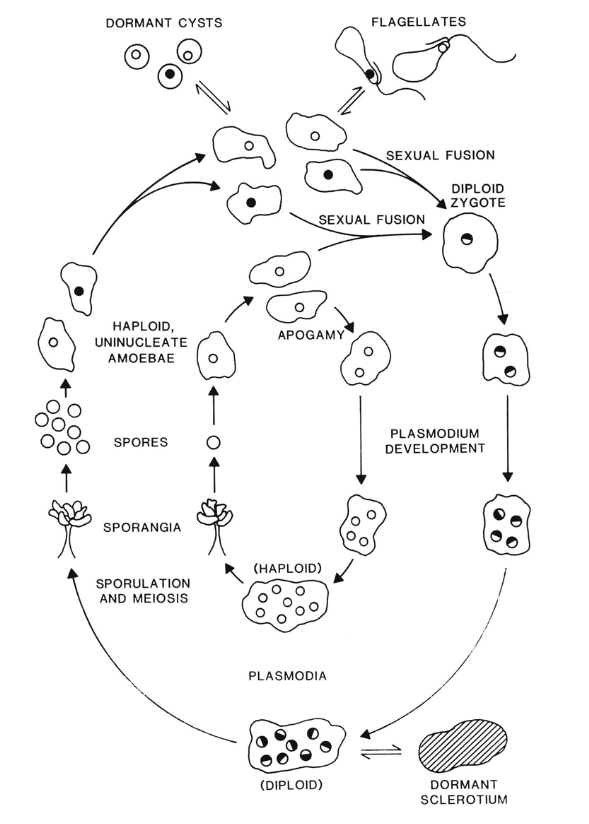
\includegraphics[width=\textwidth,height=0.9\textheight,keepaspectratio]{life_cycle.png}
			\caption[Life cycle of \P]{The complete life cycle of \Pp. Reprint from~\cite{Sauer1986}.}
			\label{fig:life_cycle}
		\end{figure}

		Next we discuss the plasmodium stage of \P in more detail as it is most relevant to this thesis.

	\subsection{The plasmodium of \textit{P. polycephalum}}

		The typical plasmodium of \P takes the shape of a tubular network. The tubes themselves are approximately cylindric and are formed by connected layers of peripheric cytoplasm. Within the tubes the internal cytoplams can freely move, transporting nuclei, nutrients and various signaling molecules. 

		\begin{figure}[ht]
			\centering
			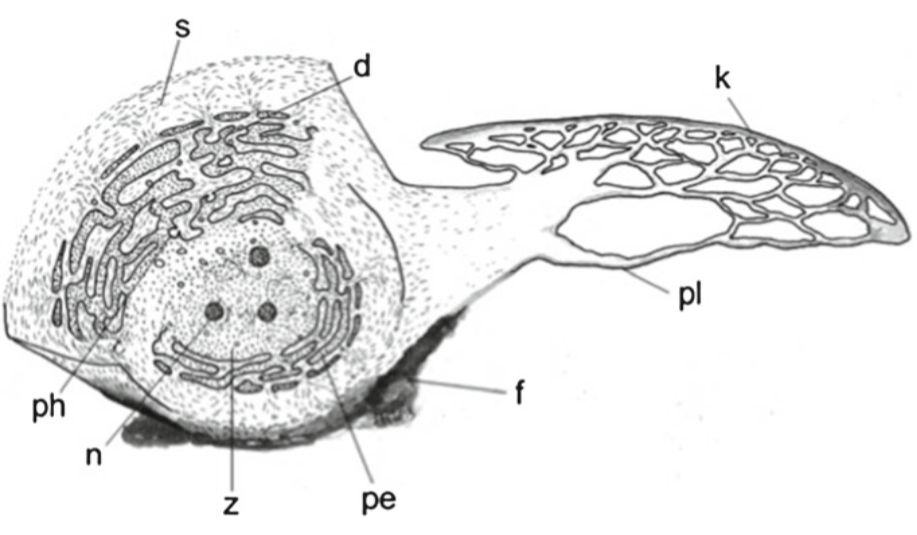
\includegraphics[width=\textwidth,height=0.9\textheight,keepaspectratio]{plasmodium_hand_drawing.png}
			\caption[Schematic drawing of the plasmodium of \P]{Schematic drawing of slime mold plasmodium with facing side sectioned and upper left section enlarged. \textbf{\texttt{k}} moving front, \textbf{\texttt{pl}} trailing plasmodial strand, \textbf{\texttt{f}} deposited material, \textbf{\texttt{s}} slime; \textbf{\texttt{d}} vacuole with deposit; \textbf{\texttt{ph}} phagocytosis vesicle; \textbf{\texttt{n}} nucleus; \textbf{\texttt{z}} central plasma; \textbf{\texttt{pe}} peripheric membrane stacks. Peristaltic contractions occur in the peripheric plasma, while the central plasma is subject to shuttle streaming. This drawing was made by Prof.~M.~Grube, Karl-Franzens Universit\"at Graz. Reprinted with permission from~\cite{grube2016physarum}.}
			\label{fig:plasmodium_hand_drawing}
		\end{figure}

		The network is highly dynamic and may change its shape in response to changing environmental conditions. This extraordinary plasticity is driven by periodic peristalsis, \ie the tubes exhibit cross-sectional contractions of Actin-Myosin fibers modulated by calcium. These contractions cause peristaltic waves and the so-called shuttle streaming of cytoplasm that can be observed in the entire network. The direction of the streaming reverses every $50 \pm 5$ seconds and reaches flow speeds up to $1000$ $\mu m/s$\footnote{Flow speeds of $2-78 \mu m/s$ known for streaming plasma in plants pale in comparison.}. These enormous speeds facilitates efficient transport of nutrients and signaling molecules across the entire organism. The wave length of the peristaltic wave depends on the size of the organism in such a way, that the net transport of cytoplasm moves the organism forward by extending its boundary. \Fref{fig:plasmodium_hand_drawing} shows a schematic drawing of a macro plasmodium.

		Provided abundant food supply, \P extends rapidly by advancing a coherent and dense apical zone, which is supported by an extended tubular network via peristaltic pumping. The growing front advances as one large unit following an exploration strategy aptly termed \emph{phalanx}, \Fref{fig:exploration:lab}. If nutrients are scarce, however, a different strategy is employed and \P tends to grow separate distinct branches each advancing its own substantially smaller growing front. This behavior allows an effective search for more distant sources of nutrients. Since branches may be guided individually by chemical attractant a more adaptive search of can be conducted. Once new food sources are found, the organism can concentrate its movement towards them. This strategy has been termed \emph{guerilla}. \Fref{fig:exploration:forest} illustrate that the plasmodium of \P may naturally interpolate between the two extreme strategies.

		We remark at this point that the phalanx and guerrilla exploration are reminiscent of two well know graph traversal strategies: Breadth-first and Depth-first search. In BSF, the explored region grows uniformly like a wave that expands evenly in all available directions. In contrast to that, DFS choose one direction in order to explore it to maximum depth. Then it backtracks to resolve the places that were ignored so far.


	\subsection{Research on Physarum}

		\P develops exceptionally well when cultured in the lab which makes it an ideal subject for scientific studies. Significant research activity in the beginning of the latter half of the 20th century explored the life cycle of \P and described the morphology and physiology of its various stages for the first time. Culturing procedures as well as genetic and molecular techniques were developed that allowed a detailed study of its mitotic cycle, cellular motility, differentiation and many other questions of biological interest. Although interest in \P was at first exclusively fueled by general questions of Biology, the scientific community soon began to appreciate the value of \P as multi-potent model system that could be controlled and studied effectively. Within a short period \P became a core experimental platform, driving various research efforts. The study of cell motility is particularly noteworthy in this context. Relevant reviews dating from the 80th can be found in~\cite{dove1980growth, aldrich2012cell,sauer1982developmental,Sauer1986}.

		After a period of intense efforts up to the 80th, the remainder of the century saw a general decline in interest in \P. It should not end until the beginning of the 21th century, when exciting new question surrounding the networks formed by the plasmodium of \P began to move into focus\footnote{Some members of the research community today humorously refer to these events as ``the second coming'' of \P.}. In particular, it was shown that these vein networks exhibit highly localized dynamic oscillatory behavior and a capability to adaptively change their topology. Together with its remarkable chemotactic abilities, these properties play a key role in the foraging behavior of \P. Despite the lack of any centralized control, they enable the organism to act as an organized unit in order to establish robust and effective vein networks connecting a potentially large set of spatially distributed food sources. In a similar context, the vein network established by \P has been shown experimentally to mimic man-made transportation networks such as railway systems or highways~\cite{tero2010rules,tero2006physarum,nakagaki2004smart}. Furthermore, it has been demonstrated that the plasmodium of \P can establish the shortest path between a pair of food sources placed in a maze~\cite{nakagaki2000intelligence}. These astounding feats received major interest amongst scientists of many disciplines and earned \P a place in the perception of the general public. Within a short period of time, \P became the focus of diverse interdisciplinary research efforts, engaging Biologists, Physicists and Computer Scientists alike. The renewed multi-disciplinary interest lead to a resurgence of research in \P that can be observed to date. For a rare more recent review and a selected recent results see~\cite{ueda2005intelligent} and~\cite{takamatsu2009environment,shirakawa2007emergence,alim2013random,tero2007mathematical,nakagaki2004obtaining}.

		Today, unraveling the global network dynamics of \P remains one of the major challenges of \P research. The emergence of effective global behavior from the delicate interplay of local effects such as oscillations, topological dynamics and the integration of chemotatctic signals is not fully understood. 



		\todo[inline]{maybe we could use some figures of the maze and the TR experiment?}




